\documentclass[11pt]{standalone}
\usepackage{amssymb}
\usepackage{amsmath}
\usepackage[no-math]{fontspec}
\usepackage{unicode-math}
\setmainfont{Libertinus Sans}
\setsansfont{Libertinus Sans}
\setmathfont{Libertinus Math}
\usepackage{pgf,xcolor}
\usepackage{tikz}
\usetikzlibrary{arrows.meta, backgrounds, calc, angles}
\usepackage{pgfplots}
\pgfplotsset{compat=newest}

\definecolor{my_darkgray}{HTML}{484949}
\definecolor{my_lightgray}{HTML}{F3F4F4}
\definecolor{my_darkblue}{HTML}{005A94}
\definecolor{my_lightblue}{HTML}{CCDEE9}
\definecolor{my_red}{HTML}{E60000}
\definecolor{my_orange}{HTML}{E87846}

\begin{document}
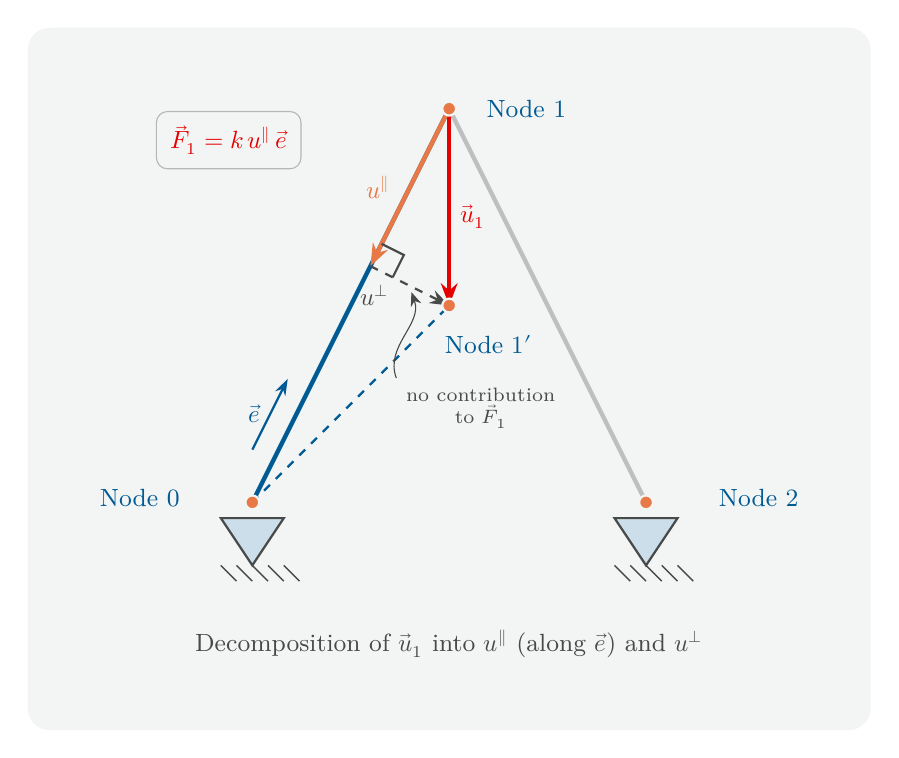
\begin{tikzpicture}[
    show background rectangle,
    background rectangle/.style={fill=my_lightgray, rounded corners=8pt},
    inner frame sep=0.8cm,
    annotation/.style={draw=my_darkgray, thin, -{Stealth[length=5pt, width=4pt]}}
]

    %------------------------------------------------------------
    % Koordinaten (Schaukelgestell aus chap04_stabgeometrie,
    % hier skaliert mit Faktor 2.5)
    %------------------------------------------------------------
    % Stab 0: N0=(0,0) -> N1=(2.5,5), e = (1,2)/sqrt(5)
    % Verschiebung u_1 = (0,-2.5) (stark überhöht)  ->  N1p = (2.5,2.5)
    % u^∥ (skalar) = dot(u_1, e) = -sqrt(5) ≈ -2.24 (Verkürzung)
    % u^∥ (vektor) = (-1, -2)  ->  Foot = (1.5, 3), liegt auf dem Stab
    % u^⊥ (vektor) = u_1 - u^∥ = (1, -0.5)
    \coordinate (N0)   at (0,   0  );
    \coordinate (N1)   at (2.5, 5  );
    \coordinate (N2)   at (5,   0  );
    \coordinate (N1p)  at (2.5, 2.5);
    \coordinate (Foot) at (1.5, 3  );

    %------------------------------------------------------------
    % Stab 1-2: dezent grau (nicht im Fokus)
    %------------------------------------------------------------
    \draw[draw=my_darkgray!35, ultra thick] (N1) -- (N2);

    %------------------------------------------------------------
    % Unverformter Stab 0-1
    %------------------------------------------------------------
    \draw[draw=my_darkblue, ultra thick] (N0) -- (N1);

    %------------------------------------------------------------
    % Einheitsvektor e: kurzer Pfeil parallel zum Stab, links versetzt
    %------------------------------------------------------------
    \draw[draw=my_darkblue, thick, -{Stealth[length=6pt, width=4pt]}]
        (0, 0.67) -- (0.45, 1.57)
        node[midway, left, font=\small, text=my_darkblue] {$\vec{e}$};

    %------------------------------------------------------------
    % Verformter Stab (gestrichelt)
    %------------------------------------------------------------
    \draw[draw=my_darkblue, thick, dashed] (N0) -- (N1p);

    %------------------------------------------------------------
    % Verschiebungsvektor u_1 (rot): N1 -> N1p
    %------------------------------------------------------------
    \draw[draw=my_red, ultra thick, -{Stealth[length=8pt, width=6pt]}]
        (N1) -- (N1p)
        node[pos=0.55, right, font=\small, text=my_red] {$\vec{u}_1$};

    %------------------------------------------------------------
    % Parallele Komponente u^∥ (orange): N1 -> Foot, auf der Stabachse
    %------------------------------------------------------------
    \draw[draw=my_orange, ultra thick, -{Stealth[length=8pt, width=6pt]}]
        (N1) -- (Foot)
        node[midway, left, font=\small, text=my_orange, xshift=-3pt] {$u^{\parallel}$};

    %------------------------------------------------------------
    % Senkrechte Komponente u^⊥ (grau, gestrichelt): Foot -> N1p
    %------------------------------------------------------------
    \draw[draw=my_darkgray, thick, dashed, -{Stealth[length=7pt, width=5pt]}]
        (Foot) -- (N1p)
        node[pos=0.3, below left, font=\small, text=my_darkgray,
             xshift=2pt, yshift=1pt] {$u^{\perp}$};

    %------------------------------------------------------------
    % Rechter Winkel bei Foot
    %------------------------------------------------------------
    \pic[draw=my_darkgray, thick, angle radius=9pt]
        {right angle = N1p--Foot--N1};

    %------------------------------------------------------------
    % Knotenpunkte
    %------------------------------------------------------------
    \foreach \P in {N0, N1, N2, N1p} {
        \draw[fill=my_orange, draw=my_lightgray, thick] (\P) circle (2.5pt);
    }

    %------------------------------------------------------------
    % Lager an Knoten 0 (linkes Festlager)
    %------------------------------------------------------------
    \draw[fill=my_lightblue, draw=my_darkgray, thick]
        (-0.4,-0.2) -- (0.4,-0.2) -- (0,-0.8) -- cycle;
    \foreach \x in {-0.4,-0.2,0,0.2,0.4} {
        \draw[draw=my_darkgray, line width=0.5pt] (\x,-0.8) -- ++(0.2,-0.2);
    }

    %------------------------------------------------------------
    % Lager an Knoten 2 (rechtes Festlager)
    %------------------------------------------------------------
    \draw[fill=my_lightblue, draw=my_darkgray, thick]
        (5.4,-0.2) -- (4.6,-0.2) -- (5,-0.8) -- cycle;
    \foreach \x in {4.6,4.8,5.0,5.2,5.4} {
        \draw[draw=my_darkgray, line width=0.5pt] (\x,-0.8) -- ++(0.2,-0.2);
    }

    %------------------------------------------------------------
    % Knotenbeschriftungen
    %------------------------------------------------------------
    \node[font=\small, text=my_darkblue, anchor=east]
        at ($(N0)+(-0.8,0.05)$) {Node 0};
    \node[font=\small, text=my_darkblue, anchor=west]
        at ($(N1)+(0.35,0)$) {Node 1};
    \node[font=\small, text=my_darkblue, anchor=west]
        at ($(N2)+(0.8,0.05)$) {Node 2};
    \node[font=\small, text=my_darkblue, anchor=north]
        at ($(N1p)+(0.5,-0.25)$) {Node $1'$};

    %------------------------------------------------------------
    % Stabkraft-Formel
    %------------------------------------------------------------
    \node[draw=my_darkgray!40, fill=my_lightgray, rounded corners=4pt,
          font=\small, text=my_red, inner sep=5pt]
        at (-0.3, 4.6)
        {$\vec{F}_1 = k\,u^{\parallel}\,\vec{e}$};

    %------------------------------------------------------------
    % Annotation: kein Beitrag (Pfeil auf u^⊥ von unten)
    %------------------------------------------------------------
    \node[font=\scriptsize, text=my_darkgray, align=center]
        (nocontrib) at (2.9, 1.2) {no contribution\\to $\vec{F}_1$};
    \draw[annotation] (nocontrib.north west) to[out=110, in=-70]
        ($(Foot)!0.5!(N1p)+(0.02,-0.08)$);

    %------------------------------------------------------------
    % Titel
    %------------------------------------------------------------
    \node[font=\small, text=my_darkgray, anchor=north]
        at (2.5,-1.5) {Decomposition of $\vec{u}_1$ into $u^{\parallel}$ (along $\vec{e}$) and $u^{\perp}$};

\end{tikzpicture}
\end{document}
